\section*{Series de Tiempo}

\subsection*{Introducción}
Muchos autores han escrito sobre las series de tiempo, pero es difícil agregar al tema o discutir las ideas del profesor Robert Hyndman, uno de los expertos más respetados en la comunidad de la estadística por su trabajo en las series de tiempo. Hyndman extiende la teoría a las series de tiempo como elementos de pronostico y su relación con la regresión lineal \cite{hyndman}. Desde el punto de vista técnico, Hyndman es el creador de varias bibliotecas de funciones de pronostico utilizando series de tiempo y ARIMA en lenguaje R. Dentro de la bibliografía, Daroczi es quien agrega detalles sobre la detección temprana de valores atípicos que pueden dificultar – y mucho – el análisis \cite{daroczi}.

\subsection*{Introducción a las Series de Tiempo}
Las series de datos son muy útiles para pronosticar algo que cambia con el tiempo. Ejemplos de estas cantidades que varían con el tiempo incluyen acciones en la bolsa de valor, cifras de ventas, y otro tipo de información cuantitativa \cite{hyndman}.

Una serie de tiempo es una serie de datos indexada en orden temporal. Comúnmente una serie de datos es una secuencia de datos tomados a puntos sucesivos y equidistantes en el tiempo, lo que la convierte en una secuencia de datos discretos en el tiempo. En forma general cualquier cosa que observamos secuencialmente en el tiempo es una serie de tiempos \cite{hyndman}. La literatura académica se concentra en series de tiempo que se observan en intervalos regulares de tiempo, aunque aquellas que se observan en intervalos irregulares también existen.

El análisis de las series de tiempo es el uso de métodos para extraer estadísticas interesantes y otras características de los datos. El pronóstico de series de tiempo es el uso de modelos para predecir valores futuros basados en valores observados en el pasado. En el pronóstico de series de tiempo, la idea principal es estimar cómo la secuencia de observaciones continuará en el futuro. El pronóstico de series de tiempo utiliza solamente información de la variable a ser pronosticada, y no hace intento alguno de descubrir cuales son los factores que motivan este comportamiento (en análisis de regresión diríamos que buscamos las variables de confusión). Por lo tanto el análisis de series de tiempo extrapola la tendencia secular y los patrones cíclicas, pero ignora todo otro tipo de información que puede afectar el movimiento de la variable estudiada, como pueden ser en la vida real efectos de la publicidad en el lanzamiento de un producto, la tasa de cambio en las ventas, o actividades de riesgo en el precio internacional de materias primas.

Podemos ver un ejemplo de serie de tiempo si tomamos los valores de la TRM (la Tasa Representativa de Mercado, el nombre oficial de la tasa de cambio del dólar en Colombia) en la siguiente gráfica:\\

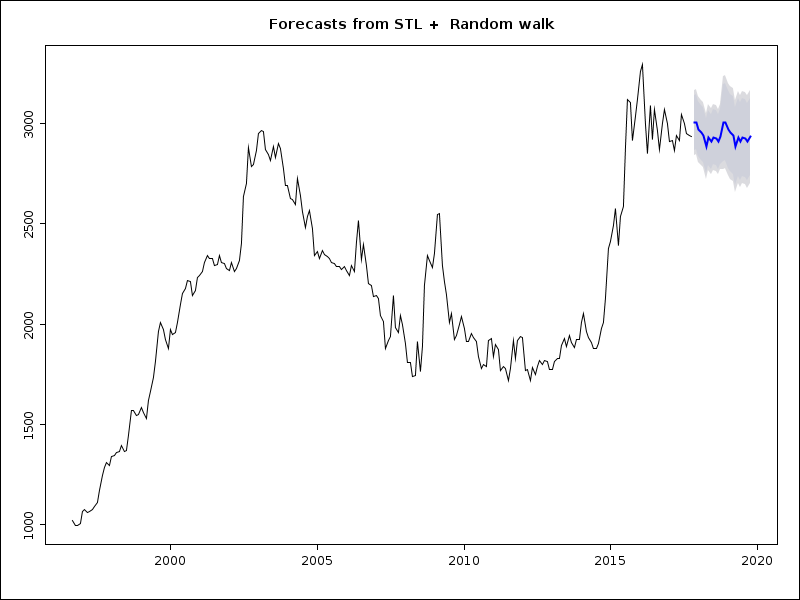
\includegraphics[width = 4 in]{timeSeries1.png}\\

La línea negra es la variación de la TRM a lo largo del tiempo (en este caso, desde el año 1980 hasta el 2017). La línea azul es el pronóstico del valor de la TRM según la función \texttt{forecast()} del lenguaje R. La zona gris comprenden el intervalo de confianza del pronóstico, la cual nos da una idea más real de como puede fluctuar el pronóstico dentro del mismo.

La forma de una ecuación de series de tiempo se puede escribir en los siguientes términos:

\[ x(t+1) = f(x_t, x_{t-1}, x_{t-2}, \ldots, error) \]

Es posible utilizar predictores en el pronóstico de series de tiempo. Un ejemplo utilizando el tema de investigación de este mismo trabajo es el pronóstico de la TRM, la cual estimamos es el resultado de varios factores:

\[ TRM = f(\textnormal{demanda dólar, tasa interés, turismo, error}) \]

La relación no es exacta, sino que siempre habrá factores por lo cuales el modelo no puede responder. Estas variaciones están previstas en el término error dentro del modelo. Este tipo de modelo se llama \emph{modelo explanatorio}.

Las series de tiempo se suelen catalogar en aditivas y multiplicativas.

\begin{itemize}
	\item Las series aditivas son aquellas cuya variación en la estacionalidad, o variación en el ciclo o tendencia secular, no aumentan de forma proporcional al avance del tiempo.
	\item Las series multiplicativas son aquellas cuya variación en la estacionalidad, o variación en el ciclo o tendencia secular, aumentan de forma proporcional al avance del tiempo. Las series multiplicativas son comunes en ciencias como la economía y finanzas.
\end{itemize}

\subsection*{Pronóstico con Series de Tiempo}
Los pronósticos con series de tiempo utilizan solamente la información disponible de la variable que se propone pronosticar, sin hacer intento alguno por descubrir los factores adicionales que condicionan su comportamiento. Por lo tanto se extrapolan las tendencias y patrones temporales, pero se ignora toda la información adicional como pueden ser iniciativas de publicidad, actividad de la competencia, cambios en las condiciones económicas y otros \cite{hyndman}.

\subsection*{Patrones}
Las series de tiempo pueden descomponerse según su patrón o tendencia en tres elementos que las componen [Velazco, M., 2017]. A saber:

\begin{enumerate}
	\item Tendencia Secular: la tendencia secular o tendencia a largo plazo de una serie de tiempo es por lo común el resultado de factores a largo plazo. La tendencia no tiene porque ser lineal. Además es común ver que la tendencia cambia de dirección, ascendente o descendente \cite{hyndman}.
	\item Variación Estacional: Es el componente de la serie de tiempo que representa la variabilidad de los datos debido a la influencia de las estaciones. El componente de estacionalidad es siempre fijo \cite{hyndman}
	\item Variación Irregular: Esta variación se debe a factores a corto plazo, imprevisibles, y no recurrentes que afectan la serie de tiempo. Algunos autores llaman a estas variaciones \emph{cíclicas}.
\end{enumerate}

Es importante saber distinguir entre los patrones cíclicos y estacionales. Los patrones estacionales tienen una duración fija y conocida en su extensión, mientras que los patrones cíclicos son mucho más extensos que los patrones estacionales y la duración de su magnitud es variable. La forma más sencilla es identificar los ciclos de estación con el calendario, por ejemplo los aumentos de tráfico en los centros comerciales en las fiestas de fin de año \cite{hyndman}.

\subsection*{Auto Correlación}
De igual manera que una correlación mide la extensión de una relación linear entre dos variables, la autocorrelación mide la relación linear entre dos valores retrasados de series de tiempo \cite{hyndman}.

El valor de una autocorrelación para un \(r_{k}\) dado es:

\[ r_{k} = \frac{\sum_{t = k + 1}^T(y_{t} - \bar{y})(y_{t - k} - \bar{y})}{\sum_{t = 1}^T(y_{t} - \bar{y})^{2}} \]

donde \(T\) es el valor de período temporal de la serie de tiempo.

El autor Daroczi agrega como metodología para la verificación de autocorrelación en un juego de datos (no solo una serie de tiempos, sino cualquier juego de datos espacial) el \emph{Indice I de Moran} \cite{daroczi}. Dicho índice esta dado por la formula:

\[ I = \frac{N}{W}
	\frac{\sum{i}\sum{j}w_{ij}(x_{i} - \bar{x})(x_{j} - \bar{x})}{{\sum{i}(x_{i} - \bar{x})^2}} \]

Los coeficientes de autocorrelación se visualizan a través de un gráfico de la función de autocorrelación o ACF (también llamado correlograma). Dicho gráfico analiza las relaciones entre valores retrasados de la serie de tiempo. Podemos utilizar la serie de tiempo representativa de la TRM para visualizar su gráfica de ACF.

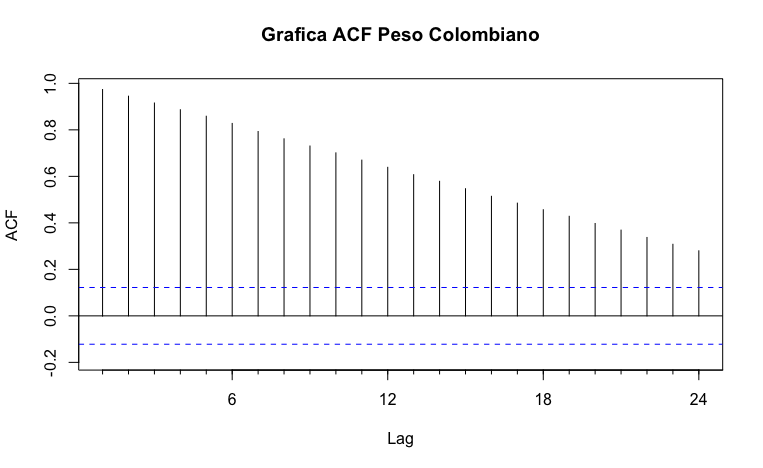
\includegraphics[width = 4 in]{COPEjemploACF.png}\\

Las series de tiempo que no muestran efectos de autocorrelación se denominan \emph{ruido blanco}. En dichas series se espera que los coeficientes de correlación sean cercanos a cero. Esto de por si es difícil, ya que toda serie de tiempo tendrá cierta variación aleatoria, pero en términos matemáticos esperamos que la serie tenga variaciones que 95\% del tiempo estén dentro de la región de $\pm2/\sqrt{T}$ donde $T$ es la extensión de la serie de tiempo. Si hay una o más series de magnitud fuera de estos límites, o si el 5\% o más de las series están fuera de estos límites, es muy probable que no sea ruido blanco \cite{hyndman}.

Existe una prueba adicional de autocorrelación que utiliza todo un grupo de datos $r_k$ en vez de tratarlos por separado. El racional para el proceso es que la visualización normal de una gráfica ACF es un test de hipótesis para cada retraso entre series. Cuando se hacen múltiples de estos test, la probabilidad de encontrar un falso positivo incrementa. Se evita este problema evaluando si las autocorrelación de los primeros $h$ valores es diferente de una serie de ruido blanco. El test de un grupo de valores con autocorrelación se conoce como un test \emph{portmanteau}. Uno de los más utilizados es el test \emph{Box-Pierce}:

\[ Q = T \sum_{k=1}^{h}r_{k\prime}^2 \]

donde $h$ es el retraso máximo considerado y $T$ es el número de observaciones. Si cada uno de los $r_k$ es cercano a cero, entonces Q sera mínimo. Si alguno de los valores de $r_k$ son grandes (ya sea positivos o negativos), entonces Q será grande. Hyndman y Athanasoupulos sugieren utilizar $h = 10$ para data no estacional y $h = 2m$ para datos con estacionalidad, donde $m$ es el número de estaciones, por ejemplo 4 para trimestres \cite{hyndman}.  El test \emph{Box-Pierce} tiende a no ser confiable con valores grandes de $h$. Si $h > T/5$ es recomendable utilizar $h=T/5$.

Un test relacionado - y más preciso - es el test \emph{Ljung-Box}:

\[ Q* = T(T+2) \sum_{k=1}^{h}(T-k)^{-1}r_{k\prime}^{2} \]

Si el valor de $Q*$ es grande, las autocorrelaciones no provienen de una serie de ruido blanco.

\subsection*{Precisión del Pronóstico}
Para el estudio de la precisión del pronóstico de series de tiempo, sea $y_i$ la observación $i$ de datos y $\hat{y_i}$ el pronóstico de $y_i$.

\subsubsection{Errores dependiente de la Escala}
El error del pronóstico es la diferencia $e_i = y_i - \hat{y_i}$, que está en la misma escala que los datos. Las medidas de precisión que dependen de $e_i$ son dependientes de la escala y no se pueden utilizar para hacer comparaciones entre series de tiempo de diferentes escalas. Las dos formas que se utilizan comúnmente para medir la precisión del pronóstico de series de tiempo dependiente de escalas están basadas en el error absoluto o error cuadrático \cite{hyndman}. Se trata de:

\begin{eqnarray*}
	\text{Error Promedio Absoluto (MAE)}& = &\text{promedio}(|e_{i}|) \\
	\text{Error Promedio Cuadrático (RMSE)}& = &\sqrt{promedio_{e_1}^2}
\end{eqnarray*}

La tendencia al comparar precisión en un solo juego de datos es utilizar el MAE ya que es mas sencillo y simple de entender.

\subsubsection{Errores Porcentuales}
Un error porcentual es del tipo $p_i = 100 e_i / y_i$. Los errores porcentuales son independientes de la escala, y se utilizan con facilidad para comparar errores en la precisión de múltiples juegos de datos. Es error porcentual más común es:

\[ \text{Error Promedio Porcentual Absoluto (MAPE)} = promedio(\mid p_i \mid) \]

Las medidas basadas en errores porcentuales tienen la debilidad de ser infinitas o indefinidas cuando $y_i = 0$ para cualquier $i$. Esto también ocurre cuando un $y_i$ tiende a cero.

\subsection{Descomposición de Series de Tiempo}
La descomposición de las series de tiempo facilita el análisis y la investigación exploratoria de los datos. Una de las formas mas sencillas de lograr esto es la aplicación de promedios móviles, lo cual se facilita mucho en R con el uso de la función \texttt{decompose()} \cite{daroczi}.

Pensemos en la serie de tiempo $y_t$ compuesta por tres factores: un componente estacional, un componente de tendencia (que contiene tanto tendencia secular como cíclica) y un último componente que contiene cualquier otro resto de información importante. Podemos entonces escribir una serie de tiempos aditiva como:

\[ y_t = S_t + T_t + E_t \]

donde $y_t$ es la data en el período $t$, $S_t$ es el componente estacional en el período $t$, $T_t$ es el componente de tendencia-ciclo en el período $t$, y $E_t$ es el componente de error en el período $t$. De forma alternativa podemos escribir una ecuación similar para los modelos de series de datos multiplicativos como:

\[ y_t = S_t * T_t * E_t  \]

El modelo aditivo es más apropiado si la magnitud de las fluctuaciones estacionales o la variación alrededor del ciclo o tendencia no varía con los niveles de la serie de tiempo (ejemplo: el avance del tiempo). Cuando la variación se da, o sea es proporcional con el avance del tiempo en la serie, un modelo multiplicativo es más apropiado. Este es el caso de la mayoría de las series de tiempo en la economía \cite{hyndman}.

\subsubsection{Datos Ajustados Estacionalmente}
Si el componente de estacionalidad se elimina de la serie de datos original, los valores resultantes se denominan \emph{ajustados estacionalmente}. Para un modelo aditivo, el ajuste por estacionalidad se da por $y_t - S_t$. Para un modelo multiplicativo este se da por $y_t/S_t$. Si la variación por estacionalidad no es de importancia, la serie ajustada por estacionalidad puede ser útil. Estos casos se dan por ejemplo con los datos de desempleo mensual, los cuales se saben tienen variación estacional que altera la lectura real del cambio.

\subsection{Métodos de Descomposición de Series de Tiempo}
Existen múltiples métodos de descomposición de series de tiempo. En nuestro marco teórico tocaremos brevemente los de promedios móviles, promedios móviles ponderados, STL, suavizar exponencialmente, y ARIMA.

\subsubsection{Promedios Móviles}

El método de promedios móviles origina de los años 1920 y fue ampliamente utilizado hasta los 1950. Hasta el día de hoy es la base de todos los otros métodos modernos de descomposición. El fundamento del mismo es utilizar los promedios móviles para estimar la tendencia o ciclo \cite{hyndman}. La descomposición por promedios móviles toma la forma siguiente:

\[ \hat{T}_{t} = \frac{1}{m} \sum_{j = -k}^{k} y_{t + j}  \]

donde $m=2k+1$. Esto significa que el estimado de la tendencia/ciclo en el momento $t$ se obtiene promediando los valores de la serie de tiempo dentro de $k$ períodos de $t$ valores.

\subsubsection{Promedios Móviles Ponderados}
Es posible obtener promedios móviles de los promedios móviles. Combinaciones de estos nos dan promedios ponderados. Por ejemplo un modelo 2X4-MA, que es un promedio de promedios móviles, es el equivalente a un modelo 5-MA con ponderaciones dadas por el vector de pesos $[\frac{1}{8}, \frac{1}{4}, \frac{1}{4}, \frac{1}{4}, \frac{1}{8}]$ \cite{hyndman}. La forma de escribir un modelo de promedios móviles ponderados es la siguiente:

\[ \hat{T}_{t} = \sum_{j = -k}^{k} a_j y_{t + j}  \]

donde $k=(m-1)/2$ y los pesos están dados por $[a_{-k}, \ldots, a_{k}]$. Es importante que todos los pesos sumen uno como valor y que sean simétricos para que $a_{j} = a_{-j}$. Una ventaja mayor de los promedios móviles ponderados es que producen estimados más suavizados de la tendencia/ciclo.

\subsubsection{Descomposición STL}
El método STL es muy versátil y robusto para la descomposición de series de tiempo. Su nombre es el acrónimo en inglés de \emph{Seasonal and Trend Descomposition using Loess}, que significa descomposición de estacionalidad y tendencia utilizando Loess. Loess es un método para estimar relaciones no-lineales desarrollado por Cleveland et al \cite{hyndman}. Las desventajas de STL es su manejo de cierta data financiera (como por ejemplo días de comercio bursátil) y las variaciones de calendario. La biblioteca de R tiene una función que descompone automáticamente una serie de datos utilizando STL, la función \texttt{STL()}.

La descomposición STL se utiliza más que nada para estudiar las series de tiempo, pero tiene aplicación en pronosticar. Asumiendo una descomposición aditiva, la serie de tiempo descompuesta se puede escribir como:

\[ y_{t} = \hat{S}_t + \hat{A}_t \]

donde $\hat{A}_t = \hat{T}_t + \hat{E}_t$ es el componente ajustado por estacionalidad. Si se trata de una serie multiplicativa entonces la misma ecuación se puede escribir como:

\[ y_{t} = \hat{S_t}\hat{A_t}\]

donde $\hat{A}_t = \hat{T}_t\hat{E}_t$.

Para pronosticar cualquier componente ajustado por estacionalidad, se puede utilizar cualquier método de pronóstico no estacional. Por ejemplo, se puede aplicar camino aleatorio con deriva, Holts-Winter, o ARIMA.

\subsubsection{Alisamiento Exponencial}
El Alisamiento Exponencial (o Suavizamiento Exponencial según la traducción), fue propuesto por Brown, Holt y Winters entre los años 1950 a 1960. Los pronósticos producto del suavizamiento exponencial son promedios ponderados de observaciones históricas en las cuales el valor del peso va decayendo a medidas que las observaciones van envejeciendo. En otras palabras, las observaciones más nuevas reciben mayor asociación con el peso.

La primera forma de suavizamiento exponencial se llama \emph{suavizamiento exponencial simple}. Este método es aplicable para el pronóstico de series de datos sin tendencia o estacionalidad. El pronostico se calcula con promedios ponderados donde los pesos decrecen exponencialmente a medida que las observaciones envejecen - los pesos más pequeños se asocian con las observaciones más antiguas.

\[ \hat{y}_{T+1 \mid T} = \alpha y_{T} + \alpha(1-\alpha) y_{T-1} + \alpha(1-\alpha)^2 y_{T-2} + \alpha(1-\alpha)^3 y_{T-3} + \ldots \]

donde $0 \leq \alpha \leq 1$ es el parámetro de alisamiento. El pronóstico de $T + 1$ es el promedio ponderado de todas las observaciones en la serie $y_1, \ldots, y_T$. La tasa por la cual decrecen los pesos se controla con el parámetro $\alpha$.

Este método se puede extender aplicando el factor de suavizamiento exponencial decreciente para lograr la ecuación de la segunda forma de suavizamiento exponencial ponderado de tal forma que:

\[ \hat{T}_{T+1 \mid T} = \sum{j=0}^{T-1} \alpha(1-\alpha)^j y_{T-j} + (1-\alpha)^{T} \ell_{0}  \]

Notemos que la ecuación es otra forma de escribir la notación del suavizamiento exponencial simple.

Holt extendió el método de suavizamiento exponencial para permitir hacer pronósticos con datos que contenían tendencia \cite{hyndman}. Este método de pronóstico incluye una ecuación de pronóstico y dos ecuaciones de suavizamiento, una para el nivel y otra para la tendencia:

\begin{eqnarray*}
	\text{Ecuación de Pronóstico}&&\hat{y}_{t+h \mid t} = \ell_{t} + hb_{t} \\
	\text{Ecuación de Nivel}&&\ell_{t} = \alpha y_{t} + (1 - \alpha)(\ell_{t-1} + b_{t-1}) \\
	\text{Ecuación de Tendencia}&&b_{t} = \beta^{*}(\ell_{t} - \ell_{t-1}) + (1 - \beta^{*})b_{t-1}
\end{eqnarray*}

donde $\ell_{t}$ denota el nivel estimado de la serie de tiempo en el momento $t$, $b_{t}$ denota el estimado de la tendencia de la serie de tiempo en el momento $t$, $\alpha$ es el parámetro de suavizamiento para el nivel, $0 \lq \alpha \leq 1$ y $\beta^{*}$ es el parámetro de suavizamiento de la tendencia, $0 \leq \beta^{*} \leq 1$.

Holt y Winters volverían sobre el método de Holt para extenderlo y capturar el elemento de estacionalidad, el único que faltaba en la ecuación. El método \emph{Holt-Winters} está compuesto por una ecuación de pronóstico y tres de suavizamiento - una para el nivel $\ell_{t}$, una para la tendencia $b_{t}$, y otra para el componente estacional $S_t$, con los parámetros de suavizamiento $\alpha$, $\beta^{2}$, y $\gamma$. Se utiliza $m$ para definir el período de estacionalidad, por ejemplo el número de temporadas en el año. De tal forma los meses serían $m=12$.

Hay dos variaciones del método que difieren en la naturaleza de los componentes de estacionalidad. El método aditivo es preferible cuando las variaciones de estacionalidad son más o menos constantes a través de la serie. El método multiplicativo es preferible cuando la variación de estacionalidad son cambiantes proporcionalmente al nivel de las series.

Los componentes de la forma aditiva son los siguientes:

\begin{equation}
\begin{split}
	\hat{y}_{t+h \mid t} & = \ell_{t} + hb_{t} + s_{t-m+h_{m}^{+}} \\
 	\ell_{t} & = \alpha(y_{t} - s_{t-m}) + (1 - \alpha)(\ell_{t-1} + b_{t-1}) \\
    b_{t} & = \beta^{*}(\ell_{t} - \ell_{t-1}) + (1 - \beta^{*})b_{t-1} \\
    s_{t} & = \gamma(y_{t} - \ell_{t-1} - b_{t-1}) + (1-\gamma)s_{t-m}
\end{split}
\end{equation}

donde $h_{m}^{+} = \lfloor (h-1) mod m \rfloor + 1$, son los que regulan que el estimado de los índices estacionales usados para el pronóstico vengan del año final de la serie. La ecuación de nivel nuestra el promedio ponderado entre la observación ajustada por estacionalidad $(y_{t} - s_{t-m}$ y el pronóstico no ajustado $(\ell_{t-1} + b_{t-1})$ para el momento $t$. La ecuación de la tendencia es idéntica al método lineal de Holt. La ecuación de la estacionalidad muestra un promedio ponderado el índice estacional actual, $(y_{t} - \ell_{t-1} - b_{t-1})$, y el índice para la misma temporada en el período previo (por ejemplo, $m$ períodos atrás).

Los parámetros de la ecuación $\ell_{t}$, $b_{t}$ y $s_{t}$ se corrigen por error dentro de la ecuación de suavizamiento con las siguientes fórmulas:

\begin{equation}
\begin{split}
	\ell_{t} & = \ell_{t-1} + b_{t-1} + \alpha e_{t} \\
    b_{t} & = b_{t-1} + \alpha \beta^{*} e_{t} \\
    s_{t} & = s_{t-m} + \gamma e_{t} \\
\end{split}
\end{equation}

Los componentes del método \emph{Holt-Winters} para modelos multiplicativos son los siguientes:

\begin{equation}
\begin{split}
	\hat{y}_{t+h \mid t} & = (\ell_{t} + hb_{t}) s_{t-m+h_{m}^{+}} \\
 	\ell_{t} & = \alpha \frac{y_{t}}{s_{t-m}} + (1 - \alpha)(\ell_{t-1} + b_{t-1}) \\
    b_{t} & = \beta^{*}(\ell_{t} - \ell_{t-1}) + (1 - \beta^{*})b_{t-1} \\
    s_{t} & = \gamma \frac{y_{t}}{(\ell_{t-1} - b_{t-1})} + (1-\gamma)s_{t-m}
\end{split}
\end{equation}

Las ecuaciones para la corrección de errores son las siguientes:

\begin{equation}
\begin{split}
	\ell_{t} & = \ell_{t-1} + b_{t-1} + \alpha \frac{e_{t}}{s_{t-m}} \\
    b_{t} & = b_{t-1} + \alpha \beta^{*} frac{e_{t}}{s_{t-m}} \\
    s_{t} & = s_{t} + \gamma frac{e_{t}}{(\ell_{t-1} + b_{t-1})} \\
\end{split}
\end{equation}

donde $e_{t} = y_{t} - (\ell_{t-1} + b_{t-1})s_{t-m}$.

\subsection{ARIMA}
Los modelos ARIMA son otro enfoque para el pronóstico de series de tiempo. Mientras que la metodología de suavizamiento exponencial busca la descripción de la tendencia y estacionalidad de la data, los modelos ARIMA intentan describir la autocorrelación de la misma.

\subsubsection{Series de Tiempo Estacionarias}
Un requisito para el modelar pronósticos con series de tiempo es que las mismas deben ser estacionarias \cite{srivastava}. Por lo tanto es importante definir la estacionalidad de series de tiempo antes de avanzar con la descomposición de las mismas.

Definimos una serie de tiempo estacionaria como aquella cuyas propiedades no dependen del momento en la cual se la observa \cite{hyndman}. Por lo tanto las series de tiempo con tendencias, o con estacionalidad, no son estacionarias. La tendencia o la estacionalidad afectará el valor de la serie de tiempos en momentos específicos de la misma. Una serie de ruido blanco es un caso de series de tiempo estacionarias. En casos puede ser confuso determinar que es que. Una serie de tiempos puede ser cíclica y estacionaria si cumple con la condición de no tener tendencia o estacionalidad.

Hay tres criterios básicos que debe cumplir una serie de tiempos para catalogarla como estacionaria \cite{srivastava}:

\begin{enumerate}
	\item El promedio de la serie no debiera ser una función del tiempo sino una constante. Esto es visible a la vista en una serie de tiempos que permanece relativamente horizontal sobre el eje de la abscisa a pesar de fluctuar.
	\item La varianza de la serie no debiera ser una función del tiempo. Esta propiedad se conoce en matemática como \emph{homocedasticidad}.
    \item La covarianza del término $x_i$ y el término $(x + m)_i$ no debiera ser una función en el tiempo. Esto también posible de ver en una gráfica, a medida que la función disminuye la distancia entre sus ondas, o aumenta la densidad de las mismas proporcional avanza en el tiempo.
\end{enumerate}

El académico Tavish Srivastava agrega sobre el concepto de series estacionarias la necesidad de asociar el de \emph{random walk} o camino aleatorio. Una serie de tiempo es un camino aleatorio con promedio cero pero con varianza dependiente en el tiempo, por lo tanto no es una serie estacionaria \cite{srivastava}.

\subsubsection{Diferenciando Series de Tiempo}
Una forma de convertir una serie de tiempo en estacionaria es diferenciarla. Al diferenciarla, se toma las diferencias entre observaciones consecutivas de la serie. La diferenciación ayuda a estabilizar el promedio de una serie de tiempos removiendo cambios en el nivel de la misma y eliminando - o por lo menos reduciendo - se tendencia y estacionalidad \cite{hyndman}.

Para una serie de tiempos estacionaria, su ACF disminuirá a cero relativamente rápido, mientras que el cuadro ACF de una serie no estacionaria disminuirá de forma paulatina y lenta. Además, para una serie no estacionaria, su valor $r_1$ es por lo general grande y positivo \cite{hyndman}.

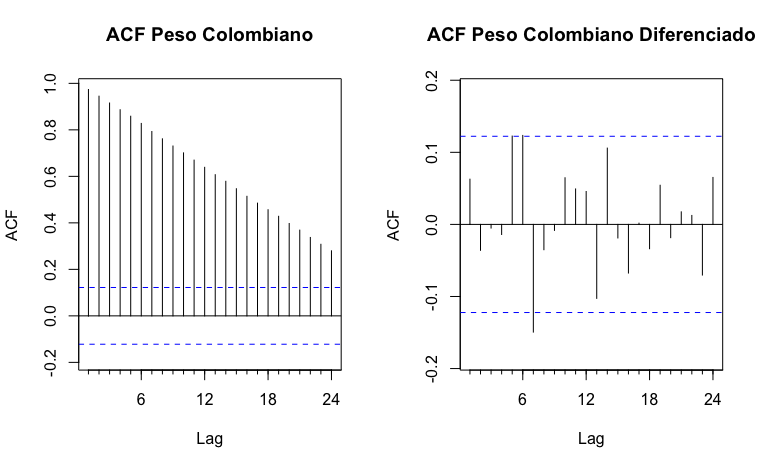
\includegraphics[width = 4 in]{DiffEjemploACF.png}\\

Una serie diferenciada es el cambio entre dos observaciones consecutivas y puede detallarse de la siguiente forma:

\[ y_{t}^{\prime} = y_{t} - y_{t-1} \]

Una serie diferenciada tendrá solo $T-1$ valores dado que no es posible calcular la diferencia $y_{1}^{\prime}$ para la primera observación. Cuando la serie diferenciada es ruido blanco, se la puede definir como:

\[ y_{t} = y_{t-1} - e_{t} \]

Las diferenciaciones también pueden hacerse por temporadas. Una diferenciación estacional es la diferencia entre una observación y su observación correspondiente del período pasado:

\[ y_{t}^{\prime} = y_{t} - y_{t-m} \]

donde $m$ es igual al número de temporadas. Estas se conocen como \emph{diferencias de m-retrasos}.

\subsubsection{Pruebas de Raíz Unitaria}
Una forma de determinar más objetivamente si hay necesidad de diferenciar una serie es la \emph{prueba de raíz unitaria}. Estas son pruebas de hipótesis estadísticas que están diseñadas para determinar la necesidad o no de diferenciación de la serie \cite{hyndman}. Existen varias y están basadas en diferentes enfoques, por lo que es común utilizar más de una si hay respuestas conflictivas que confrontar.

La más utilizada es la prueba aumentada \emph{Dickey-Fuller}, también conocida como \emph{ADF}. Para este test, se utiliza el siguiente modelo de regresión \cite{dickeyfuller}:

\[ y_{t}^{\prime} = \phi y_{t-1} + \beta y_{t-1}^{\prime} + \beta_{2} y_{t-2}^{\prime} + \ldots + \beta_{k} y_{t-k}^{\prime} \]

donde $y_{t}^{\prime}$ denota la primera serie diferenciada, $y_{t}^{\prime} = y_{t} - y_{t-1}$ y $k$ es el número de retrasos para incluir en la regresión (que por regla común se ajusta a 3). Si la serie original, $y_{t}$, necesita diferenciarse, entonces el coeficiente $\hat{\phi}$ debiera aproximar a cero. Si $y_{t}$ ya es estacionaria, $\hat{\phi} < 0$. La metodología normal de test de hipótesis no funciona cuando la serie es estacionaria, pero el lenguaje \emph{R} tiene una función que lo calcula sin problemas de la forma \texttt{adf.test(x, alternative="stationary")} \cite{packageForecast}.

La hipótesis nula para una prueba \emph{Dickey-Fuller} es que la data es no-estacionaria. De tal manera que valores grandes de $p$ son indicativos de no-estacionalidad y valores pequeños de $p$ por el contrario indican que la hipótesis alternativa es de serie estacionaria. Un corolario de esto es que se necesita usar diferenciación cuando $p > 0.05$.

\subsubsection{Modelos Autoregresivos (AR)}
En un modelo de regresión múltiple, pronosticamos la variable de interés usando una combinación lineal de predictores. En un modelo autoregresivo, el pronóstico de la variable de interés se conforma con una combinación lineal de valores pasados de la variable. El término autoregresión indica que es una regresión de variables contra si mismas \cite{hyndman}.

Por lo tanto un modelo autogresivo de orden $p$ puede ser escrito como:

\[ y_{t} = c + \phi_{1}y_{t-1} + \phi_{2}y_{t-2} + \ldots + \phi_{p}y_{t-p} + e_{t}  \]

donde $e_{t}$ es ruido blanco. Es muy similar a la regresión múltiple pero con valores retrasados de $y_{t}$ como predictores. Esto se refiere a un modelo \textbf{AR(p)}. Los modelos autoregresivos son muy flexibles para manejar un portafolio amplio de patrones de series de datos. El cambio de los parámetros $\phi_1, \ldots, \phi_{p}$ resulta en diferentes patrones de series de datos. La varianza del término de error $e_t$ solo modifica la escala de la serie, no los patrones.

\subsubsection{Modelos de Promedios Móviles (MA)}
En vez de utilizar los valores pasados de una variable de pronóstico en una regresión, el modelo de promedios móviles utiliza los errores pasados del pronóstico en un modelo cuasi-regresión.

\[ y_{t} = c + e_{t} + \phi_{1}e_{t-1} + \phi_{2}e_{t-2} + \ldots + \phi_{q}e_{t-q} \]

donde $e_{t}$ es ruido blanco. Nos referimos a este modelo como \textbf{MA(q)}. En realidad no observamos los valores de $e_{t}$, por lo que no es una regresión en el sentido estricto de la palabra \cite{hyndman}. Hacemos notar que cada valor de $y_{t}$ puede ser pensado como un promedio móvil ponderado de los últimos errores de pronóstico. Sin embargo no hay que confundirlo con el suavizamiento de promedios móviles. El cambio de los parámetros $\phi_1, \ldots, \phi_{p}$ resulta en diferentes patrones de series de datos. Al igual que en los modelos autoregresivos, la variación del término de error $e_t$ solo modifica la escala de la serie, no los patrones.

\subsubsection{Modelos ARIMA No-Estacionarios}
Si combinamos la diferenciación con la autoregresión y un modelo de promedios móviles, obtenemos el \emph{modelo no-estacionario ARIMA}. ARIMA es el acrónimo para \emph{AutoRegressive Integrated Moving Average} (o modelos autoregresivos integrados de promedios móviles). En este caso son integrados porque la integración es la función opuesta de diferenciación \cite{hyndman}. Podemos escribir el modelo completo como:

\[ y_{t}^{\prime} = c + \phi_{1}y_{t-1}^{\prime} + \ldots + \phi_{p}y_{t-p}^{\prime} + \phi_{1}e_{t-1} + \ldots + \phi_{q}e_{t-q} + e_{t} \]

donde $y_{t}^{\prime}$ es la serie diferenciada (puede haber sido diferenciada más de una vez). Los predictores en la mano derecha de la ecuación incluyen tanto valores rezagados de $y_t$ y errores rezagados. A esto lo llamamos un modelo \textbf{ARIMA(p, d, q)}, donde:

\begin{description}
  \item [p = ]
  orden de la parte autoregresiva;
  \item [d = ]
  grado de la primera diferenciación involucrada;
  \item [q = ]
  orden de la parte de promedios móviles.
\end{description}

Las mismas condiciones de estacionalidad e invertibilidad que se utiliza en los modelos de autoregresión y promedios móviles aplican al modelo ARIMA.

\subsubsection{Gráficas ACF y PACF}
Seleccionar el juego indicado de variables \emph{p, d, q} puede ser difícil. Las bibliotecas de \emph{R} tienen funciones para ayudar. Por lo general no es posible a simple vista evaluar estos valores. Sin embargo, si es posible utilizar las gráficas de la función de autocorrelación ACF y su función asociada PACF para seleccionar valores de \textit{p} y \textit{q}. La gráfica de la función PACF mide la autocorrelación parcial entre $y_{t}$ y $y_{t-k}$ después de eliminar los efectos de otras series rezagadas $1, 2, 3, \ldots, k-1$. Por lo tanto la primer autocorrelación parcial es idéntica a la primer autocorrelación, porque no hay nada que eliminar.

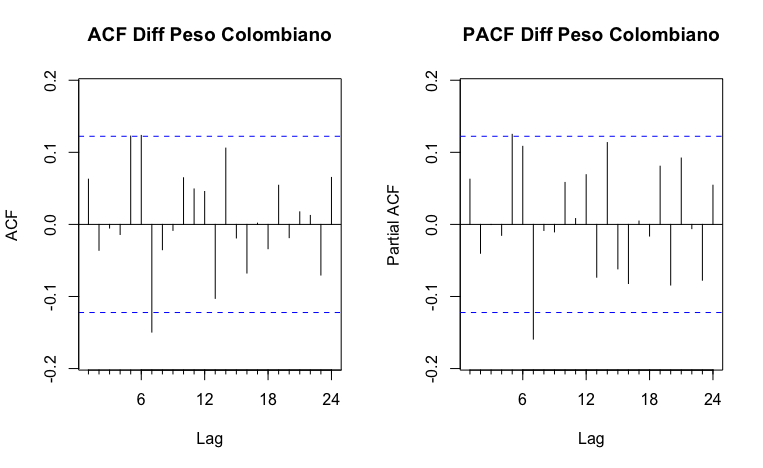
\includegraphics[width = 4 in]{ACFPACFEjemplo.png}\\

Si los datos son de un modelo \textit{ARIMA(p,d,0)} o \textit{ARIMA (0,d,q)}, entonces las gráficas ACF y PACF pueden ser útiles en determinar los valores de \emph{p} o \emph{q}. Si tanto \emph{p} y \emph{q} son positivas, los gráficos no podrán ayudar a determinar los valores adecuados de \emph{p} y \emph{q}.

Los datos pueden seguir un modelo ARIMA(p,d,0) si el gráfico ACF y PACF de los datos diferenciados muestran los siguientes patrones.
\begin{itemize}
	\item la gráfica ACF decrece exponencialmente o tiene forma sinusoide
	\item hay un crecimiento significativo en el tramo \textit{p} en la gráfica PACF, pero ninguno después del tramo \textit{p}
\end{itemize}

Los datos pueden seguir un modelo ARIMA(0,d,q) si el gráfico ACF y PACF de los datos diferenciados muestran los siguientes patrones.
\begin{itemize}
	\item la gráfica PACF decrece exponencialmente o tiene forma sinusoide
	\item hay un crecimiento significativo en el tramo \textit{p} en la gráfica ACF, pero ninguno después del tramo \textit{p}
\end{itemize}
